%\documentclass[journal]{IEEEtran}
%\documentclass[draft]{IEEEtran}
\documentclass[onecolumn,draftclsnofoot]{IEEEtran}

\usepackage[utf8]{inputenc}
\usepackage{amsmath}
\usepackage{amsfonts}
\usepackage{amssymb}
\usepackage{amsthm}
\usepackage{graphicx}
\usepackage{todonotes}
\usepackage{natbib}
\usepackage{url}
\usepackage[boxruled,vlined,linesnumbered]{algorithm2e}
\usepackage{caption}
\usepackage{subcaption}
\usepackage{lineno}
\usepackage{tcolorbox}
\usepackage{hyperref}
\AtBeginDocument{\let\textlabel\label}
\hypersetup{colorlinks=true,linkcolor=black,citecolor=black,filecolor=black,urlcolor=black}


\captionsetup[figure]{labelfont=it,textfont={it},textfont=footnotesize}
\captionsetup[subfigure]{width=0.8\hsize,labelfont=bf,textfont=footnotesize,singlelinecheck=off,justification=raggedright,format=hang}

\theoremstyle{definition}
\newtheorem{definition}{Definition}



\author{Jonathan Rosenblatt \\ 
	Department of IE\&M and \\
	Zlotowsky Center for Neuroscience, \\
	Ben Gurion University of the Negev, Israel. 
	\and Jelle Goeman \\ 
	Department of Medical Statistics and Bioinformatics, \\
	Leiden University Medical Center, The Netherlands.
	\and Roee Gilron \\ Tel Aviv University,
	\and Roy Mukamel \\ Tel Aviv University.}


%% OPTIONAL MACRO DEFINITIONS
%\def\s{\sigma}
\newcommand{\set}[1]{\{ #1 \}} % A set
\newcommand{\indicator}[1]{\mathcal{I}{\set{#1}}} % The indicator function.
\newcommand{\reals}{\mathbb{R}} % the set of real numbers
\newcommand{\xS}{\mathcal{X}} % The feature space
\newcommand{\yS}{\mathcal{Y}} % The feature space
\newcommand{\expect}[1]{\mathbf{E}\left[ #1 \right]} % The expectation operator
\newcommand{\acc}{\mathcal{E}} 
\newcommand{\accEstim}{\hat{\mathcal{E}}} 
\newcommand{\accZ}{\hat{\mathcal{Z}}} 
\newcommand{\hyp}{\algo_{\data}} % A hypothesis
\newcommand{\hypFun}[2]{\algo_{#1}(#2)} % A hypothesis
\newcommand{\hypEstim}{\algo(\data)} %{\hat{\hyp}} % A hypothesis
\newcommand{\hypclass}{\mathcal{F}}
\newcommand{\prob}[1]{Prob( #1 )} % the probability of an event
\newcommand{\rv}[1]{\mathbf{#1}} % A random variable
\newcommand{\x}{\rv x} % The random variable x 
\newcommand{\y}{\rv y} % The random variable x 
\newcommand{\X}{\rv X} % The random variable x 
\newcommand{\Y}{\rv Y} % The random variable y
\newcommand{\gauss}[1]{\mathcal{N}\left(#1\right)} % The Gaussian distribution
\newcommand{\gaussp}[2]{\mathcal{N}_{#1}\left(#2\right)} % The Gaussian distribution
\newcommand{\mycaption}{Simulation details in Section\ref{sec:simulation_details}, except the changes in the sub-captions.}
\newcommand{\argmin}[2]{\mathop{argmin} _{#1}\set{#2}} % The argmin operator
\newcommand{\argmax}[2]{\mathop{argmax} _{#1}\set{#2}} % The argmin operator
\newcommand{\R}{\textsf{R }}
\newcommand{\algo}{\mathcal{A}}
\newcommand{\data}{\mathcal{S}}
\newcommand{\measure}{\mathcal{P}}
\newcommand{\measuren}{\measure_\data}
\newcommand{\union}{\cup}
\newcommand{\intersect}{\cap}
\newcommand{\majority}{\accEstim_{Maj}}
\newcommand{\statistic}{\mathcal{T}}




% correct bad hyphenation here
\hyphenation{op-tical net-works semi-conduc-tor}


\begin{document}
\title{Better-Than-Chance Classification for Signal Detection}
%
%
% author names and IEEE memberships
% note positions of commas and nonbreaking spaces ( ~ ) LaTeX will not break
% a structure at a ~ so this keeps an author's name from being broken across
% two lines.
% use \thanks{} to gain access to the first footnote area
% a separate \thanks must be used for each paragraph as LaTeX2e's \thanks
% was not built to handle multiple paragraphs
%

\author{Jonathan~D.~Rosenblatt,~\IEEEmembership{}
        Yuval~Benjamini,~\IEEEmembership{}
        Roee~Gilron,~\IEEEmembership{}
        Roy~Mukamel,~\IEEEmembership{}
        and~Jelle~J.~Goeman,~\IEEEmembership{}%

\thanks{JDR was supported by the ISF 900/60 research grant.}% <-this % stops a space
\thanks{JDR and J. Doe are with Anonymous University.}% <-this % stops a space
\thanks{Manuscript received April 19, 2005; revised August 26, 2015.}}

% note the % following the last \IEEEmembership and also \thanks - 
% these prevent an unwanted space from occurring between the last author name
% and the end of the author line. i.e., if you had this:
% 
% \author{....lastname \thanks{...} \thanks{...} }
%                     ^------------^------------^----Do not want these spaces!
%
% a space would be appended to the last name and could cause every name on that
% line to be shifted left slightly. This is one of those "LaTeX things". For
% instance, "\textbf{A} \textbf{B}" will typeset as "A B" not "AB". To get
% "AB" then you have to do: "\textbf{A}\textbf{B}"
% \thanks is no different in this regard, so shield the last } of each \thanks
% that ends a line with a % and do not let a space in before the next \thanks.
% Spaces after \IEEEmembership other than the last one are OK (and needed) as
% you are supposed to have spaces between the names. For what it is worth,
% this is a minor point as most people would not even notice if the said evil
% space somehow managed to creep in.



% The paper headers
\markboth{}%
{Rosenblatt \MakeLowercase{\textit{et al.}}: Classification for Signal Detection}
% The only time the second header will appear is for the odd numbered pages
% after the title page when using the twoside option.



% If you want to put a publisher's ID mark on the page you can do it like
% this:
%\IEEEpubid{0000--0000/00\$00.00~\copyright~2015 IEEE}
% Remember, if you use this you must call \IEEEpubidadjcol in the second
% column for its text to clear the IEEEpubid mark.



% use for special paper notices
%\IEEEspecialpapernotice{(Invited Paper)}




% make the title area
\maketitle

% As a general rule, do not put math, special symbols or citations
% in the abstract or keywords.
\begin{abstract}
The estimated accuracy of a classifier is a random quantity with variability. 
A common practice in supervised machine learning, is thus to test if the estimated accuracy is significantly better than chance level.
This method of signal detection is particularly popular in neuroimaging and genetics.
We provide evidence that using a classifier's accuracy as a test statistic can be an underpowered strategy for finding differences between populations, compared to a bona-fide statistical test.
It is also computationally more demanding than a statistical test. 
Via simulation, we compare test statistics that are based on classification accuracy, to others based on multivariate test statistics. 
We find that probability of detecting differences between two distributions is lower for accuracy based statistics.
We examine several candidate causes for the low power of accuracy-tests. 
These causes include: the discrete nature of the accuracy-test statistic, the type of signal accuracy-tests are designed to detect, their inefficient use of the data, and their regularization. 
When the purposes of the analysis is not signal detection, but rather, the evaluation of a particular classifier, we suggest several improvements to increase power. 
In particular, to replace V-fold cross validation with the Leave-One-Out Bootstrap.
\end{abstract}

% Note that keywords are not normally used for peerreview papers.
\begin{IEEEkeywords}
signal-detection, multivariate-testing, supervised-learning, hypothesis-testing, high-dimension.
\end{IEEEkeywords}






% For peer review papers, you can put extra information on the cover
% page as needed:
% \ifCLASSOPTIONpeerreview
% \begin{center} \bfseries EDICS Category: 3-BBND \end{center}
% \fi
%
% For peerreview papers, this IEEEtran command inserts a page break and
% creates the second title. It will be ignored for other modes.
\IEEEpeerreviewmaketitle



\section{Introduction}
\label{sec:introduction}

\IEEEPARstart{M}{any} neuroscientists and geneticists detect signal by fitting a classifier and testing whether it's prediction accuracy is better than chance. 
The workflow consists of fitting a classifier, estimating its predictive accuracy using cross validation, and test the hypothesis that this accuracy can be attributed to chance alone. 
This general idea has been promoted by \cite{friedman2003multivariate,eric2008testing,ojala_permutation_2010,lopez2016revisiting}.
Examples in the genetics literature include
\cite{golub_molecular_1999,slonim_class_2000,radmacher_paradigm_2002,mukherjee_estimating_2003,juan_prediction_2004,jiang_calculating_2008,yu2007two}.
Other examples include speaker verification \cite{gretton_kernel_2012-1}, 
text classification \cite{dhillon2003divisive,lopez2016revisiting}, distinguishing between facial expressions \cite{lopez2016revisiting}, data integration \cite{gretton_kernel_2012-1}, record linkage in databases systems \cite{gretton_kernel_2012-1,hall2002permutation,vayatis_auc_2009}, optical character recognition \cite{perez2009estimation}, multimedia \cite{moreno2004kullback}, and functional data analysis \cite{hall2002permutation}.

Examples in the neuroscientific literature, which is our motivating use-case, include \cite{golland_permutation_2003,pereira_machine_2009,schreiber2013statistical,olivetti2013kernel,varoquaux_assessing_2016}, and especially the recently popularized \emph{multivariate pattern analysis} (MVPA) framework in \cite{kriegeskorte_information-based_2006}.

To fix ideas, we will adhere to a concrete example.
In \cite{gilron_quantifying_2016}, Gilron et al. seek to detect brain regions that encode differences between vocal and non-vocal stimuli. 
Following the MVPA workflow, the localization problem is cast as a supervised learning problem: if the type of the stimulus can be predicted from the brain's activation pattern significantly better than chance, then a region is declared to encode vocal/non-vocal information. 
We call this an \emph{accuracy-test}, because it uses the prediction accuracy as a test statistic. 

This same signal detection task can also be approached as a multivariate \emph{two-group} test.
Inferring that a region encodes vocal/non-vocal information, is essentially inferring that the spatial distribution of brain activations is different given a vocal/non-vocal stimulus. 
As put in \cite{pereira_machine_2009}: 
\begin{quote}
	... the problem of deciding whether the classifier learned to discriminate the classes can be subsumed into the more general question as to whether there is evidence that the underlying distributions of each class are equal or not.
\end{quote}
A practitioner may thus approach the signal detection problem with a two-group hypothesis test.
Multivariate two-groups hypothesis-tests may be divided into tests for equality of location (i.e. means), and two-sample goodness of fit tests (i.e., equality of the two whole distribution, GOF in short).
The former generalizing the t-test, and the latter (roughly) generalizing Kolmogorov-Smirnov's test.


Crucially for our applications, we will assume that the number of samples is in the order of the dimension of each sample, if not smaller. 
In the statistical literature this is known as a \emph{high-dimensional} problem. 
We emphasize that by high-dimension it is not necessarily implied that the sample is large, even if it is often the case. 
In our motivating example it means that the size of the brain's region of interest is large compared to the number of subjects in the experiment. 
It is thus a \emph{high-dim--small-sample} problem. 

In a seminal contribution, Bai and Saranadasa \cite{bai1996effect} noted that in-high dimension, multivariate tests tend to be low powered unless some regularization is involved. 
Since then, many high-dimensional tests have been proposed. 
These can be classified along the following lines:
\begin{itemize}
	\item \textbf{High-dim GOF}: Tests that seek for any difference between two distributions, such as  \cite{hall2002permutation,szekely_brownian_2009,gretton_kernel_2012-1}.
	
	\item \textbf{High-dim location test for sparse shift}: Tests the seek for a sparse shift in mean vectors such as \cite{tony2014two,chang2014simulation}.
	
	\item \textbf{High-dim location test for dense shift}: Tests the seek for a dense shift in mean vectors such as  \cite{dempster1958high,bai1996effect,schafer_shrinkage_2005,goeman2006testing,srivastava_multivariate_2007,lopes2011more,nishiyama2013testing,thulin2014high,shen2015adaptive,xu2016adaptive,zhang2016high}.
	
	\item \textbf{High-dim location test for shift with unknown sparsity}: Tests the seek for a shift in mean vectors, but adapt to the unknown sparsity, such as \cite{donoho2004higher,zhong2013tests,moscovich2016exact}.
	
\end{itemize}

At this point, it becomes unclear which test is preferable, in particular for genetics and neuroimaging?
In this manuscript, we do not provide a full answer to the matter.
Instead, we merely seek to demonstrate that \textbf{accuracy-tests are never optimal, compared to high-dim two-group tests}.
Out recommendations to the practitioner in these high-dim problems:
(i) Prefer a two-group test over an accuracy-test. 
(ii) Appropriate regularization is crucial. 

Various authors have compared accuracy-tests to two-group tests, often with contradicting conclusions.
In \cite{yu2007two} for instance, authors find that an accuracy-test based on a tree predictor is preferable over a two-group test. 
Their simulated shift is sparse, so that it is no surprise that a tree-type predictors outperforms linear predictors and tests. 
Authors of \cite{olivetti2013kernel} compare the kernel test of Gretton et al. \cite{gretton_kernel_2012-1} to an accuracy-test based on logistic-regression.
Their results are inconclusive with a slight advantage to the logistic regression.
In \cite{lopez2016revisiting}, authors compare several accuracy-tests to several two-group tests and conclude that an accuracy-test based on a neural-net is preferable. 
Their argument is that the neural-net is able to learn the features that best separate the samples. Their examples, however, are low-dimensional (even if large-sample), and such feature learning is typically impossible in high-dimension.

Ramdas et al. \cite{ramdas_classification_2016} currently offer the only analytic comparison; comparing Hotelling's $T^2$ location test to \emph{Fisher's linear discriminant analysis} (LDA) accuracy-test. 
By comparing the rates of convergence of the power of each statistic, \cite{ramdas_classification_2016} conclude LDA and $T^2$ are rate equivalent. 
Rates, however, are only a first stage when comparing test statistics. 

Asymptotic relative efficiency measures (ARE) are typically used by statisticians to compare between rate-equivalent test statistics \cite{vaart_asymptotic_1998}.
ARE is the limiting ratio of the sample sizes required by two statistics to achieve similar power. 
The authors of \cite{ramdas_classification_2016} derive the asymptotic power functions of the two test statistics, with which we are able to compute the ARE between Hotelling's $T^2$ (two-group) test and Fisher's LDA (accuracy) test.
Theorem~14.7 of \cite{vaart_asymptotic_1998} relates asymptotic power functions to ARE.
Using this theorem and the results of \cite{ramdas_classification_2016} we deduce that the ARE is lower bounded by $2 \pi \approx 6.3$. 
This means that Fisher's LDA requires at least $6.3$ more samples to achieve the same (asymptotic) power as the $T^2$ test. 
In this light, the accuracy-test is remarkably inefficient.  
For comparison, the t-test is only $1.04$ more (asymptotically) efficient than Wilcoxon's rank-sum test \cite{lehmann_parametric_2009}, so that an ARE of $6.3$ is strong evidence in favor of the two-group test. 

The analysis in \cite{ramdas_classification_2016} is asymptotic. 
Since typical sample sizes in neuroscience and genetics are not large, we seek to study which test is to be preferred in finite samples, and not only asymptotically.
Lacking a unifying mathematical framework for the finite sample power analysis, we opt for a simulation study. 

We start with formalizing the problem in Section~\ref{sec:problem_setup}.
The main findings are reported in Sections~\ref{sec:results}, and \ref{sec:example}.
We conclude with a discussion.



%\hfill mds

%\hfill August 26, 2015



%%%% Section %%%%
\section{Problem setup}
\label{sec:problem_setup}


\subsection{Multivariate Testing}

Let $y \in \mathcal{Y}$ be a class encoding. 
Let $x \in \mathcal{X}$ be a $p$ dimensional feature vector. 
In our vocal/non-vocal example we have $\mathcal{Y}=\set{0,1}$ and $p=27$, the number of voxels in a brain region so that $\mathcal{X}=\reals^{27}$. 

We denote a sample from $x$ given $y$ with $x_y$.
We denote the distribution of $x_1$ by $\mathcal{F}$ and $x_0$ with $\mathcal{G}$.
Denoting a dataset by $\data:=\{(x_i,y_i)\}_{i=1}^n$, a two-group test amounts to testing whether $\mathcal{F}=\mathcal{G}$.
For example, we can test whether multivariate voxel activation patterns are similarly distributed when given a vocal stimulus ($x_1$) or a non-vocal one ($x_0$).
The tests are calibrated to have a fixed false positive rate ($\alpha=0.05$).
The comparison metric between statistics is power, i.e., the probability to infer that $\mathcal{F}\neq\mathcal{G}$.


\subsection{From a Test Statistic to a Permutation Test}

The multivariate tests we will be considering rely on fixing some test statistic, $\mathcal{T}$, and comparing it to it's permutation distribution. 
The tests differ in the statistic they employ.
Our comparison metric is their power, i.e., their true positive rate. 
We adhere to permutation tests and not parametric inference because in our problems of interest central limit approximations are typically poor.

Because we focus on two-group testing under an independent sampling assumption, we know that a label-switching permutation test is valid. 
The sketch of our permutation test is the following: \newline
(a) Fix a test statistic $\mathcal{T}$ with a right tailed rejection region. \newline
(b) Sample a random permutation of the class labels, $\pi(y)$. \newline
(c) Permute labels and recompute the statistic $\mathcal{T}_\pi$. \newline
(d) Repeat (a)-(c) $R$ times. \newline
(e) The permutation p-value is the proportion of  $\mathcal{T}_\pi$ larger than the observed $\mathcal{T}$. Formally: 
$\mathbb{P}\{\mathcal{T}_\pi \geq \mathcal{T}\}:=\frac{1}{R} \sum_{\pi} I\{\mathcal{T}_\pi \geq \mathcal{T}\}$.\newline
(f) Declare $\mathcal{F}\neq \mathcal{G}$ if the permutation p-value is smaller than $\alpha$, which we set to $\alpha=0.05$.
\bigskip

We now detail the various test statistics that will be compared.


\subsection{Two-Group Tests}
The most prevalent interpretation of $\mathcal{F}\neq \mathcal{G}$ is to assume they differ in means\footnote{This is not a logical equivalence, but rather a prevalent convention. The Behrnes-Fisher problem is a counter example where equal means do not imply equal distributions.}. 
Difference in means leads to the \emph{shift class} of alternatives, which is by far the most studied class in the statistical literature. 
In his seminal work in 1931, Harold Hotelling proposed the $T^2$ test as a straightforward generalization of the t-test, for testing the equality in means of two multivariate distributions \cite{hotelling_generalization_1931}. 
Hotelling's statistic was later shown to be the generalized-likelihood-ratio statistic in the Gaussian shift class. 
It can also be thought of as the empirical Mahalanobis norm of the mean difference, or the empirical Kullback–Leibler divergence between the distribution of averages from two shifted Gaussian distributions. 
For more background see, for example, \cite{anderson_introduction_2003}.

The major difficulty with the $T^2$ statistic is that it requires estimating a covariance matrix, thus introducing $p(p+1)/2=\mathcal{O}(p^2)$ unknown parameters.
If $n$ is not much larger than $p$, or in low signal-to-noise (SNR), the test is very low powered, as shown in \cite{bai1996effect}. 
In these cases, high dimensional versions of the $T^2$ should be applied, which essentially regularize the estimator of $\Sigma$, thus reducing the dimensionality of the problem and improving the SNR and power.
Examples of high-dim tests for (dense) shifts include 
\cite{dempster1958high,bai1996effect,schafer_shrinkage_2005,goeman2006testing,srivastava_test_2008,chen_two-sample_2010,lopes2011more,ahmad2014u,thulin2014high,feng2015note}.

If $\mathbb{E}(x_1)$ differs from $\mathbb{E}(x_0)$ in a small number of coordinates we say the \emph{signal is sparse}.
Examples of high-dim tests statistics for sparse shifts include \cite{cai_two-sample_2013} and \cite{chang2014simulation}.

It is possible that the practitioner is unaware of the amount of sparsity in the signal. 
Some high-dim test statistics that \emph{adapt} to the level of (unknown) sparsity include \cite{simes1986improved,donoho2004higher,zhong2013tests,shen2015adaptive,moscovich2016exact}.

It is possible that the signal is present (not only) in means. 
We would thus opt for a two-group GOF test, instead of a location test. 
Examples of multivariate GOF tests include \cite{bickel1969distribution,friedman1979multivariate,hall2002permutation,szekely2004testing,Biau2005,Rosenbaum2005,eric2008testing,perez2009estimation,vayatis_auc_2009,gretton_kernel_2012-1}.

As previously mentioned, a classifier's accuracy may also be used as a test statistic. We now explain how this an accuracy-test is constructed. 


\subsection{Prediction Accuracy as a Test Statistic}
An accuracy-test amounts to using a predictor's accuracy as a test statistic.  
A predictor\footnote{Also known as a \emph{hypothesis} in the machine learning literature.}, $\hyp:\mathcal{X} \to \mathcal{Y}$, is the output of a learning algorithm $\algo$ when applied to the dataset $\data$. 
The accuracy of predictor\footnote{Also known as (the complement of) the \emph{test error}.}, $\acc_{\hyp}$, is defined as the probability of $\hyp$ making a correct prediction. 
The accuracy of a learning algorithm\footnote{Also known  as (the complement of) the \emph{expected test error}.}, $\acc_{\algo}$, is defined as the expected accuracy over all possible data sets $\data$. 
Formalizing, we denote by $\measure$ the probability measure of $(x, y)$, and by $\measuren$ the joint probability measure of the sample $\data$. 
We can then write $\acc_{\hyp}:=\int_{(x,y)} \indicator{\hyp(x)=y} \; d\measure,$
and
$\acc_{\algo}:=\int_\data \acc_{\algo_\data} \; d\measuren,$
where $\indicator{A}$ is the indicator function\footnote{Mutatis mutandis for continuous $y$.} of the set $A$. 

Denoting an estimate of $\acc_{\hyp}$ by $\accEstim_{\hyp}$, and $\acc_{\algo}$ by $\accEstim_{\algo}$, a statistically significant ``better than chance'' estimate of either, is evidence that the classes are distinct. 
Two popular estimates of $\accEstim_{\algo}$ are the \emph{resubstitution accuracy}\footnote{Also known as (the complement of) the \emph{train error}.}, and the V-fold Cross Validation (CV) estimate.
\begin{definition}[Resubstitution accuracy]
	\label{def:resubstitution}
	The resubstitution accuracy estimator of a learning algorithm $\algo$, denoted $\accEstim_{\algo}^{Resub}$,  is defined as
$\accEstim_{\algo}^{Resub} := \frac 1n \sum_{i=1}^{n} \indicator{\hypFun{\data}{x_i}=y_i}.$
\end{definition}


\begin{definition}[V-fold CV accuracy]
	\label{def:v-fold}
	Denoting by $\data^{v}$ the $v$'th partition, or \emph{fold}, of the dataset, and by $\data^{(v)}$ its complement, so that $\data^{v} \union \data^{(v)}=\union_{v=1}^V \data^{v}=\data$, the V-fold CV accuracy estimator, denoted $\accEstim_{\algo}^{Vfold}$, is defined as 	
$\accEstim_{\algo}^{Vfold} := 
	\frac 1V \sum_{v=1}^{V} \frac{1}{|\data^v|} \sum_{i \in \data^{v}} \indicator{\hypFun{\data^{(v)}}{x_i}=y_i},$
	where $|A|$ denotes the cardinality of a set $A$.
\end{definition}




\subsection{How to Estimate Accuracies?}
\label{sec:considerations}

Estimating $\accEstim_{\algo}$ requires the following design choices: 
Should it be cross-validated and how? 
If cross validating using V-fold CV then how many folds? 
Should the folding be balanced?
If estimation is part of a permutation test: should the data be refolded after each permutation? 

We will now address these questions while bearing in mind that unlike the typical supervised learning setup, we are not interested in an unbiased estimate of $\acc_{\algo}$, but rather in the detection of its departure from chance level. 

\paragraph{Cross validate or not}
For the purpose of statistical testing, bias in $\hat\acc_{\algo}$ is not a problem, as long as it does not invalidate the error rate guarantees. 
The underlying intuition is that if the same bias is introduced in all permutations, it will not affect the properties of the permutation test. 
We will thus be considering both cross validated accuracies, and resubstitution accuracies.


\paragraph{Balanced folding}
The standard practice in V-fold CV is to constrain the data folds to be balanced, i.e. stratified \cite[for e.g.]{ojala_permutation_2010}.
This means that each fold has the same number of examples from each class. 
We will report results only with balanced folding, mostly because we will conclude that V-fold CV should not be used for our detection problem. 


\paragraph{Refolding}
In V-fold CV, \emph{folding} the data means assigning each observation to one of the $V$ data folds. 
The standard practice in neuroimaging is to permute labels and refold the data after each permutation. 
This is done because permuting labels will unbalance the original balanced folding.
We will adhere to this practice due to its popularity, even though it is computationally more efficient to permute features\footnote{The difference between permuting labels, $\pi(y)$, or features, $\pi(X)$, is in the mapping to folds. When permuting features, the \textit{label} assignment to folds is fixed. When permuting labels, the \textit{feature} assignment to folds is fixed.} instead of labels, as done by \cite{golland_permutation_2005}.


\paragraph{How many folds}
Different authors suggest different rules for the number of folds. 
We fix the number of folds to $V=4$, and do dot discuss the effect of $V$ because we will ultimately show that V-fold CV is dominated by other cross-validation procedures, and thus, never recommended. 

\bigskip

Table~\ref{tab:collected} collects an initial battery of tests we will be comparing. 
\begin{tcolorbox}
	\centering
	\footnotesize
	\begin{tabular}{l|c|c|c}
		Name & Algorithm & Resampling & Remark\\ 
		\hline
		\hline
		svm.CV.cCV 	& SVM & V-fold  & cost=CV \\ 
		svm.noCV.c001 	& SVM & Resubstitution  & cost=$0.01$ \\ 
		svm.noCV.c100 	& SVM & Resubstitution  & cost=$100$ \\ 
		svm.CV.c001	& SVM & V-fold 		    & cost=$0.01$ \\ 
		svm.CV.c100	& SVM & V-fold 		    & cost=$100$ \\ 
		lda.noCV.1 	& LDA & Resubstitution 	&  --\\ 
		lda.CV.1 	& LDA & V-fold 			&  -- \\ 
		Cai & \cite{cai_two-sample_2013} & Resubstitution & -- \\ 
		Simes & \cite{simes1986improved} & Resubstitution & -- \\ 
		dCOV & \cite{szekely2004testing} & Resubstitution & -- \\ 
		Gretton & \cite{gretton_kernel_2012-1} & Resubstitution & -- \\ 
		Srivastava & \cite{srivastava_test_2008} & Resubstitution & -- \\ 
		Goeman & \cite{goeman2006testing} & Resubstitution & -- \\ 
		Schafer & \cite{schafer_shrinkage_2005} & Resubstitution & -- \\ 
		Hotelling & $T^2$ & Resubstitution & -- \\
		Oracle & $T^2$ & Resubstitution & Known $\Sigma$\\ 
	\end{tabular} 
	\captionsetup{type=table}
	\caption{\footnotesize
		This table collects the various test statistics we will be studying. 
		Two-group tests for dense shits include: \textit{Oracle}, \textit{Hotelling}, \textit{Schafer}, \textit{Goeman}, and \textit{Srivastava}.
		Two-group tests for sparse shifts include \textit{Cai}.
		Two-group adaptive tests for shifts include \textit{Simes}.
		The rest are accuracy-tests with details given in the table. 	
		For example, \textit{svm.CV.c100} is a linear SVM, with V-fold cross validated accuracy, and cost parameter set at $100$ \cite{meyer_e1071:_2015}.
		\textit{svm.CV.cCV} is a linear SVM, with V-fold CV accuracy, and cost parameter optimized with (an inner) CV. 
		\textit{lda.noCV.1} is Fisher's LDA, with a resubstituted accuracy estimate.
		Also recall that in LIBSVM, the \emph{cost} is inversely proportional to the regularization \cite{chang2011libsvm}: larger cost=less regularization. 
		}
	\label{tab:collected}
\end{tcolorbox}





%%%% Section %%%%
\section{Results}
\label{sec:results}
We now compare the power of our various statistics in various configurations. 
We do so via simulation.
The basic simulation setup is presented in Section~\ref{sec:simulation_details}.
Following sections present variations on the basic setup.
The \R code for the simulations can be found in \url{http://www.john-ros.com/permuting_accuracy/}.


\subsection{Basic Simulation Setup and Notation}
\label{sec:simulation_details}

Each simulation is based on $1,000$ replications. 
In each replication, we generate $n$ independent samples from a shift class 
\begin{align}
\label{eq:distribution}
\x_i = \mu \y_i + \eta_i,
\end{align}
where $\y_i \in \mathcal{Y}=\set{0,1}$ encodes the class of subject $i$, $\mu$ is a $p$-dimensional shift vector, the noise $\eta_i$ is distributed as $\gaussp{p}{0,\Sigma}$, the sample size $n=40$, and the dimension of the data is $p=23$. 
The covariance $\Sigma=I$. 
In this basic setup, reported in Figure~\ref{fig:simulation_1}, the shift effect is captured by $\mu$. 
Shifts are dense and equal in all $p$ coordinates of $\mu$.
With $e$ being a $p$-vector of ones, then $\mu:=c \, e$. 
We will use $c$ to index the signal's strength, and vary it over $c \in \set{0,1/4,1/2}$.
When setting $\Sigma=I$ then the (squared) Euclidean and Mahalanobis norms of the signal are $\Vert \mu \Vert_2^2=\Vert \mu \Vert_\Theta^2=\mu' \Sigma^{-1} \mu= c^2 p\approx \{0,1.4,5.7\}$, where $\Theta:=\Sigma^{-1}$. 
These can be thought as the effect's size. 


Having generated the data, we compute each of the test statistics in Table~\ref{tab:collected}.
For test statistics that require data folding, we used $4$ folds. 
We then compute a permutation p-value by permuting the class labels, and recomputing each test statistic. 
We perform $300$ such permutations. 
We then reject the $\mathcal{F}=\mathcal{G}$ null hypothesis if the permutation p-value is smaller than $0.05$.
The reported power is the proportion of replication where the permutation p-value fell below $0.05$.



\subsection{False Positive Rate}
\label{sec:type_i}

We start with a sanity check. 
Theory suggests that all test statistics should control their false positive rate. 
Our simulations confirm this.
In all our results, such as Figure~\ref{fig:simulation_1}, we encode the null case, where $\mathcal{F}=\mathcal{G}$, by a red circle. 
Since the red circles are always below the desired $0.05$ error rate then the false positive rate of all test statistics, in all simulations is controlled. 
We may thus proceed and compare the power of each test statistic. 






%%%% Section %%%%
\subsection{Power}
\label{sec:power}

From Figure~\ref{fig:simulation_1} we learn that two-group tests are more powerful than accuracy-tests.

\begin{figure}[h]
	\centering
	\includegraphics[width=0.7\columnwidth]{"art/file2"}
	\caption{
		The power of the permutation test with various test statistics. 
		The power on the $x$ axis. 
		Effects are color and shape coded. 
		Effects vary over $c=0$ (red circle), $c=1/4$ (green triangle), and $c=1/2$ (blue square). 
		The various statistics on the $y$ axis. 
		Their details are given in Table~\ref{tab:collected}. 
		Simulation details in Section~\ref{sec:simulation_details}.}	
	\label{fig:simulation_1}
\end{figure}




\subsection{Large Sample}
\label{sec:large-sample}

We focus on high-dim--small-sample configurations because of our motivation in neuroimaging and genetics. 
Our results, however hold also in high-dim--large-sample configurations.
To prove this point, we fix $p/n$ at $23/40$, and set $n=4,000, p=2,300$. 
The results are reported in Figure~\ref{fig:large-sample}.


\begin{figure}[h]
	\centering
	\includegraphics[width=0.7\columnwidth]{"art/file1"}
	\caption{[TODO: update figure] The same as Figure~\ref{fig:simulation_1} with $n=4,000; p=2,300$.}
	\label{fig:large-sample}
\end{figure}




%
%\subsection{Tie Breaking}
%\label{sec:ties}
%
%As already stated in the introduction, the accuracy statistic is highly discrete. 
%Especially the resubstitution accuracy-tests. 
%Discrete test statistics lose power by not exhausting the permissible false positive rate. 
%A common remedy is a \emph{randomized test}, in which the rejection of the null is decided at random in a manner that exhausts the false positive rate. 
%Formally, denoting by $\mathcal{T}$ the observed test statistic, by $\mathcal{T}_\pi$, its value after under permutation $\pi$, and by $\mathbb{P}\{A\}$ the proportion of permutations satisfying $A$ then the randomized version of our tests imply that if the permutation p-value, 
%$\mathbb{P}\{\mathcal{T}_\pi \geq \mathcal{T}\}$, 
%is greater than  $\alpha$ then we reject the null with probability 
%$$ max\left\{\frac{\alpha - \mathbb{P}\{\mathcal{T}_\pi > \mathcal{T}\}}{\mathbb{P}\{\mathcal{T}_\pi = \mathcal{T}\}},0 \right\}.$$
%
%Figure~\ref{fig:file33} reports the same analysis as in Figure~\ref{fig:file2}, after allowing for random tie breaking. 
%It demonstrates that the power disadvantage of accuracy-tests, cannot be remedied by random tie breaking.
%
%\begin{figure}[ht]
%	\centering
%	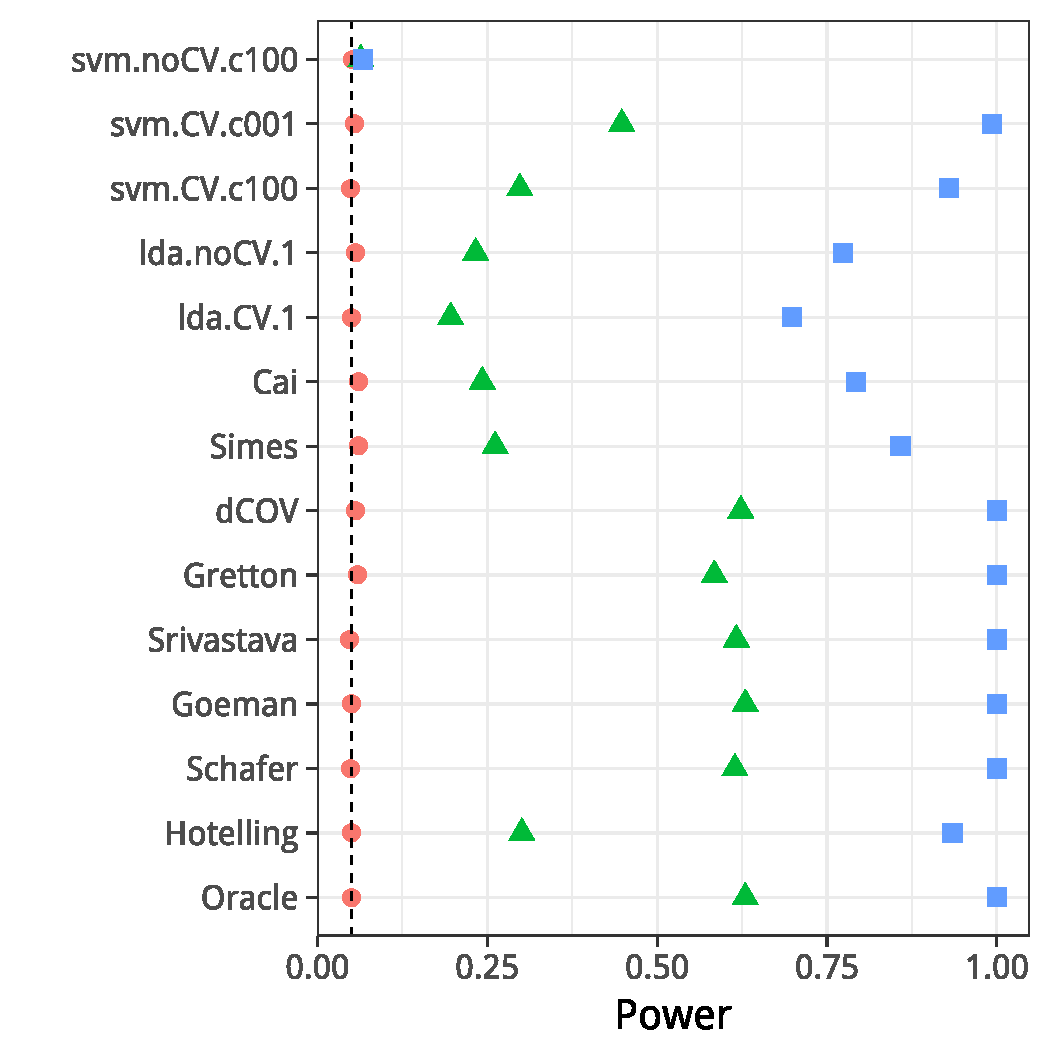
\includegraphics[width=0.7\columnwidth]{art/file33}
%	\caption{The same as Figure~\ref{fig:file2}, with random tie breaking.}
%	\label{fig:file33}
%\end{figure}
%


\subsection{Departure From Gaussianity}
The Neyman-Pearson Lemma (NPL) type reasoning that favors two-group location-tests over accuracy-tests in our simulations, may fail when the data is not multivariate Gaussian, and Hotelling's $T^2$ statistic no longer a generalized-likelihood-ratio test. 

To check this, we replaced the multivariate Gaussian distribution of $\eta$ in Eq.(\ref{eq:distribution}) with a heavy-tailed multivariate-$t$ distribution. 
In this heavytailed setup, the dominance of the two-group tests was preserved, even if less evident than in the Gaussian case (Figure~\ref{fig:t_null}).



\begin{figure}[th]
	\centering
	\includegraphics[width=0.7\columnwidth]{"art/file9"}
	\caption{\textbf{Heavytailed.} $\eta_i$ is $p$-variate t, with $df=3$ .  } 
	\label{fig:t_null}
\end{figure}




% Dependence
\subsection{Departure from Sphericity}
\label{sec:dependence}

We now test the robustness of our results to the correlations in $x$. 
In terms of Eq.(\ref{eq:distribution}), $\Sigma$ will no longer be the identity matrix. 
Almost all tests include some estimator of $\Sigma$, so that correlations should be accounted for.
Then again, estimating $\Sigma$ introduces variance, at the cost of reduced bias.
We thus have no a-priori guess on the effect of the added correlations. 
To keep the comparisons ``fair'' as the correlations vary, we kept $\Vert \mu \Vert_\Theta:=\sqrt{\mu'\Theta\mu}$ fixed.

Which test has more power: accuracy or two-group?
We address this question using various correlation structures.
We also vary the direction of the signal, $\mu$, and distinguish between signal in high variance principal component (PC) of $\Sigma$, and in the low variance PC. 

The simulation results reveal some non trivial phenomena.
First, when the signal is in the direction of the high variance PC, the high-dim two-group tests are far superior than accuracy-tests. 
This holds true for various correlation structures: the short memory correlations of $AR(1)$ in Figure~\ref{fig:dependence_11}, the long memory correlations of a Brownian motion in Figure~\ref{fig:dependence_21}, and the arbitrary correlation in Figure~\ref{fig:dependence_31}.

When the signal is in the direction of the low variance PC, a different phenomenon appears.
There is no clear preference between two-group or accuracy-tests.
Instead the non-regularized tests are the clear victors. 
This holds true for various correlation structures: the short memory correlations of $AR(1)$ in Figure~\ref{fig:dependence_12}, the long memory correlations of a Brownian motion in Figure~\ref{fig:dependence_22}, and the arbitrary correlation in Figure~\ref{fig:dependence_32}.
We attribute this phenomenon to the bias introduced by the regularization, which masks the signal.
This matter is further discussed in Section~\ref{sec:fix_snr}.

\begin{figure}[h]
	\centering
	\begin{subfigure}[t]{.45\columnwidth}
		\centering
		\includegraphics[width=1\columnwidth]{"art/file20"}
		\caption{Signal in direction of highest variance PC of $\Sigma$.} 
		\label{fig:dependence_11}
	\end{subfigure}
	\begin{subfigure}[t]{.45\columnwidth}
		\centering
		\includegraphics[width=1\columnwidth]{"art/file21"}
		\caption{Signal in direction of lowest variance PC of $\Sigma$.} 
		\label{fig:dependence_12}
	\end{subfigure}
	%	\begin{subfigure}[t]{.3\columnwidth}
	%		\centering
	%		  \includegraphics[width=1\columnwidth]{"art/file11"}
	%		\caption{Signal in direction of identity vector.} 
	%		\label{fig:dependence_13}
	%	\end{subfigure}
		\caption{Short memory, AR(1) correlation. 
			$\Sigma_{k,l}=\rho^{|k-l|}; \rho=0.6$.}
		\label{fig:dependence_1}
\end{figure}


\begin{figure}[h]
	\centering
	\begin{subfigure}[t]{.45\columnwidth}
		\centering
		\includegraphics[width=1\columnwidth]{"art/file22"}
		\caption{Signal in direction of highest variance PC of $\Sigma$.} 
		\label{fig:dependence_21}
	\end{subfigure}
	\begin{subfigure}[t]{.45\columnwidth}
		\centering
		\includegraphics[width=1\columnwidth]{"art/file23"}
		\caption{Signal in direction of lowest lowest variance PC of $\Sigma$.} 
		\label{fig:dependence_22}
	\end{subfigure}
	%	\begin{subfigure}[t]{.3\columnwidth}
	%		\centering
	%		\includegraphics[width=1\columnwidth]{"art/file16"}
	%		\caption{Signal in direction of identity vector.} 
	%		\label{fig:dependence_23}
	%	\end{subfigure}
		\caption{Long-memory Brownian motion correlation: $\Sigma=D^{-1} R D^{-1}$ where $D$ is diagonal with $D_{jj}=\sqrt{R_{jj}}$, and $R_{k,l}=\min\{k,l\}$.}	
		\label{fig:dependence_2}
\end{figure}



\begin{figure}[h]
	\centering
	\begin{subfigure}[t]{.45\columnwidth}
		\centering
		\includegraphics[width=1\columnwidth]{"art/file18"}
		\caption{Signal in direction of highest variance PC of $\Sigma$.} 
		\label{fig:dependence_31}
	\end{subfigure}
	\begin{subfigure}[t]{.45\columnwidth}
		\centering
		\includegraphics[width=1\columnwidth]{"art/file17"}
		\caption{Signal in direction of lowest variance PC of $\Sigma$.} 
		\label{fig:dependence_32}
	\end{subfigure}
	%	\begin{subfigure}[t]{.3\columnwidth}
	%		\centering
	%		\includegraphics[width=1\columnwidth]{"art/file19"}
	%		\caption{Signal in direction of identity vector.} 
	%		\label{fig:dependence_33}
	%	\end{subfigure}
		\caption{Arbitrary Correlation. 
			$\Sigma=D^{-1} R D^{-1}$ where $D$ is diagonal with $D_{jj}=\sqrt{R_{jj}}$, and $R=A'A$ where $A$ is a Gaussian $p\times p$ random matrix with independent $\mathcal{N}(0,1)$ entries.
		}
		\label{fig:dependence_3}
\end{figure}



\subsection{Departure from Homoskedasticity and Scalar Invariance}

Our previous simulations assume variables a have unit variance. 
Practitioners are already accustomed to z-score features before learning a regularized predictor (e.g. ridge regression) so this is not an unrealistic setup.
Implicit z-scoring is sometime an integral part of a test statistic. 
This is known as \emph{scalar invariance}.
The \emph{Srivastava} statistic, for instance, is scalar invariant. 
It can be (roughly) thought of as the $l_2$ norm of the $p$-vector of coordinate-wise t-statistics.
The \emph{Goeman} statistic, for instance, is not scalar invariant. 
It can be (roughly) thought of as the $l_2$ norm of the $p$-vector of variable-wise mean differences.

Under heteroskedasticity, the \emph{Goeman} statistic will give less importance to signal in the high-variance directions than signal in the low-variance directions. \emph{Srivastava} will give all coordinates the same importance.

In Figure~\ref{fig:heteroskedastic_11} we can see the difference between the scalar-invariant \emph{Srivastava} and \emph{Goeman} statistics. We also see that two-group tests dominate accuracy-tests also in the heteroskedastic case. 

\begin{figure}[h]
	\centering
	\begin{subfigure}[t]{.45\columnwidth}
		\centering
		\includegraphics[width=1\columnwidth]{"art/file26"}
		\caption{$\mu$ in the high variance PC of $\Sigma$.}  
		\label{fig:heteroskedastic_11}	
	\end{subfigure}
	\begin{subfigure}[t]{0.45\columnwidth}
		\centering
		\includegraphics[width=1\columnwidth]{"art/file24"}
		\caption{$\mu$ in the low variance PC of $\Sigma$.}  
		\label{fig:heteroskedastic_12}	
	\end{subfigure}
		\caption{Heteroskedasticity: $\Sigma$ is diagonal with $\Sigma_{jj}=j$.}	
		\label{fig:heteroskedastic}	
\end{figure}







% Resampling with replacement
\subsection{Departure from V-fold CV}
\label{sec:bootstrap}

Intuition suggests we may alleviate the discretization of the accuracy-test statistic by replacing the V-fold CV, and resampling \emph{with replacement}.
The discretization of the accuracy statistic is governed by the number of samples in the union of test sets.
For V-fold CV, for instance, the accuracy may assume $n$ values. 
This suggests that the accuracy can be ``smoothed'' by allowing the test sample to be drawn with replacement. 
An algorithm that samples test sets with replacement is the \emph{leave-one-out bootstrap estimator},  and its derivatives, such as the \emph{0.632 bootstrap}, and \emph{0.632+ bootstrap} \cite[Sec 7.11]{hastie_elements_2003}.
\begin{definition}[bLOO]
	\label{def:bloo}
	The \emph{leave-one-out bootstrap} estimate, bLOO, is the average accuracy of the holdout observations, over all bootstrap samples. 
	Denote by $\data^b$, a bootstrap sample $b$ of size $n$, sampled with replacement from $\data$. 
	Also denote by $C^{(i)}$ the index set of bootstrap samples not containing observation $i$.
	The leave-one-out bootstrap estimate, $\accEstim_{\algo}^{bLOO}$,  is defined as:
$\accEstim_{\algo}^{bLOO}:= \frac 1n \sum_{i=1}^{n} \frac{1}{|C^{(i)}|} \sum_{b \in C^{(i)}} \indicator{\hypFun{\data^b}{x_i}=y_i}.$
	An equivalent formulation, which stresses the Bootstrap nature of the algorithm is the following. 
	Denoting by $S^{(b)}$ the indexes of observations that are \emph{not} in the bootstrap sample $b$ and are not empty, 
$\accEstim_{\algo}^{bLOO} = \frac 1B \sum_{b=1}^{B} \frac{1}{|S^{(b)}|} \sum_{i \in S^{(b)}} \indicator{\hypFun{\data^b}{x_i}=y_i}.$
\end{definition}


Simulation results are reported in Figure~\ref{fig:bootstrap} with naming conventions in Table~\ref{tab:collected_2}.
As expected, sampling test sets with replacement does increase the power of accuracy-tests, when compared to V-fold cross validation, but still falls short from the power of two-group tests. 
It can also be seen that power increases with the number of bootstrap replications, since more replications reduce the level of discretization.

\bigskip

\begin{tcolorbox}
	\centering
	\footnotesize
	\begin{tabular}{l|c|c|c|c}
		Name & Algorithm & Resampling & B  & Remark\\ 
		\hline
		\hline
		lda.Boot.b10 & LDA & bLOO 	& $10$ &  -- \\ 
		svm.Boot.c001.b50 & SVM & bLOO 	& $10$ & cost=0.01 \\ 
		svm.Boot.c100.b50 & SVM & bLOO 	& $10$ & cost=100 \\ 
		svm.Boot.c001.b10 & SVM & bLOO 	& $50$ & cost=0.01 \\ 
		svm.Boot.c100.b10 & SVM & bLOO 	& $50$ & cost=100 \\ 
	\end{tabular} 
	\captionsetup{type=table}
	\caption{\footnotesize
		The same as Table~\ref{tab:collected} for bootstrapped accuracy estimates. 
		bLOO is defined in~\ref{def:bloo}.
		$B$ denotes the number of Bootstrap samples.} 
	\label{tab:collected_2}
\end{tcolorbox}


\begin{figure}[ht]
	\centering
	\includegraphics[width=0.7\columnwidth]{"art/file13"}
	\caption{
		\textbf{Bootstrap.}
		The power of a permutation test with various test statistics. 
		The power on the $x$ axis. 
		Effects are color and shape coded. 
		The various statistics on the $y$ axis. 
		Their details are given in tables~\ref{tab:collected} and \ref{tab:collected_2}. 
		Effects vary over $0$ (red circle), $0.25$ (green triangle), and $0.5$ (blue square). 
		Simulation details in Appendix~\ref{sec:simulation_details}.
	} 
	\label{fig:bootstrap}
\end{figure}






\subsection{The Effect of High Dimension}
\label{sec:highdim}

Our setup of $n=40$ and $p=23$ is high-dim--small-sample, which surfaces finite-sample effects, not manifested in low-dim, $p/n \to 0$ asymptotic analysis.
Our best performing tests alleviate the dimensionality of the problem by regularizing the estimation of $\Sigma$. 
Shrinking, or thresholding the entries of $\hat{\Sigma}$ reduces variance at the cost of some (possible) bias. 
We know that this regularization increases power, just by comparing the non-regularized $T^2$ to its regularized versions. 
Can we do the same for classifiers? 
To answer this question we augment the comparison with some accuracy-tests that have explicit covariance regularization in them. 
These include shrinkage based LDA \cite{pang_shrinkage-based_2009,ramey_high-dimensional_2016}, where Tikhonov regularization of $\hat \Sigma$ is used; just like the \emph{Schafer} statistic.
We also try we try a diagonalized LDA~\cite{dudoit_comparison_2002}, also known as \emph{Gaussian Na\"ive Bayes}, which regularizes similarly to the \emph{Srivastava} and \emph{Goeman} statistics.

Simulation results are reported in Figure~\ref{fig:highdim} with naming conventions in Table~\ref{tab:collected_3}.
The proper regularization of the covariance of a classifier, just like a two-group test, can improve power. 
See, for instance, \emph{svm.CV.c001} which is clearly the best regularized SVM for testing. 
Replacing the V-fold  with a bootstrap allows us to further increase the power, as done with \emph{lda.highdim.Pang.b50}.
Even so, the out-of-the-box two-group tests outperform the accuracy-tests.

It is interesting to note that \emph{svm.CV.cCV} is not a good performer. 
In SVMs, the cost parameter governs the magnitude of the margins, and thus the regularization. 
In \emph{svm.CV.cCV} this regularization is optimized with CV which leads us to argue that the optimal regularization for prediction is not the same as the optimal for testing.

\bigskip

\begin{tcolorbox}
	\centering
	\footnotesize
	\begin{tabular}{l|c|c|c}
		Name & Algorithm & Resampling &  Parameters\\ 
		\hline
		\hline
		lda.highdim.Dudoit.CV & \cite{dudoit_comparison_2002} & V-fold & -- \\ 
		lda.highdim.Ramey.CV & \cite{ramey_high-dimensional_2016} & V-fold & -- \\ 
		lda.highdim.Pang.CV & \cite{pang_shrinkage-based_2009} & V-fold & -- \\ 
		lda.highdim.Pang.b50 & \cite{pang_shrinkage-based_2009} & bLOO 	 & B=50 \\ 
	\end{tabular} 
	\captionsetup{type=table}
	\caption{\footnotesize
		The same as Table~\ref{tab:collected} for regularized (high dimensional) predictors. 
	} 
	\label{tab:collected_3}
\end{tcolorbox}


\begin{figure}[ht]
	\centering
	\includegraphics[width=0.7\columnwidth]{"art/file14"}
	\caption{[TODO: sync figure with names in table]
		\textbf{HighDim Classifier.} 
		The power of a permutation test with various test statistics. 
		The power on the $x$ axis. 
		Effects are color and shape coded. 
		The various statistics on the $y$ axis. 
		Their details are given in tables~\ref{tab:collected} and \ref{tab:collected_3}. 
		Effects vary over $0$ (red circle), $0.25$ (green triangle), and $0.5$ (blue square). 
		Simulation details in Section~\ref{sec:simulation_details}.
	} 
	\label{fig:highdim}
\end{figure}








%%%%%%%   Neuroimaging
\section{Neuroimaging Example}
\label{sec:example}

Figure~\ref{fig:read_data} is an application of the Srivastava two-group test, and a linear SVM accuracy-test, to the neuroimaging data of \cite{pernet_human_2015}. 
The authors of \cite{pernet_human_2015} collected fMRI data while subjects were exposed to the sounds of human speech (vocal), and other non-vocal sounds. 
Each subject was exposed to $20$ sounds of each type, totaling in $n=40$ trials.
The study was rather large and consisted of about $200$ subjects.
The data was kindly made available by the authors at the OpenNeuro website\footnote{\url{http://reproducibility.stanford.edu/}}.

We perform group inference using within-subject permutations along the analysis pipeline of \cite{stelzer_statistical_2013}, which was also reported in \cite{gilron_quantifying_2016}. 

In agreement with our simulation results, the two-group test (\emph{Srivastava}) discovers more brain regions of interest when compared to an accuracy-test.
The former discovers $1,232$ regions, while the latter only $441$, as depicted in Figure~\ref{fig:read_data}.
We emphasize that both test statistics were compared with the same permutation scheme, and the same error controls, so that any difference in detections is due to their different power.


\begin{figure}[th]
	\centering
	\includegraphics[width=1\columnwidth]{"art/svm_vs_SD"}
	\caption{\footnotesize
		Brain regions encoding information discriminating between vocal and non-vocal stimuli.
		Map reports the centers of $27$-voxel sized spherical regions, as discovered by an accuracy-test u and a two-group test (\emph{Srivastava}). 
		The linear SVM was computed using $5$-fold cross validation, and a cost parameter of $1$. 
		Region-wise significance was determined using the permutation scheme of \cite{stelzer_statistical_2013}, followed by region-wise $FDR \leq 0.05$ control using the Benjamini-Hochberg procedure \cite{benjamini_controlling_1995}.
		Number of permutations equals $400$.
		The two-group test detect $1,232$ regions, and the accuracy-test $441$, $399$ of which are common to both.
		For the details of the analysis see \cite{gilron_quantifying_2016}.  
	}
	\label{fig:read_data}
\end{figure}








%%%% Section %%%%
\section{Discussion}
\label{sec:discussion}

We have set out to understand which of the tests is more powerful: accuracy-tests or two-group tests. 
Our current observation is that in various setups, accuracy-tests are never optimal in high-dim; there is always a two-group test that dominates in power.
We conjecture that they are never optimal, simply because of the needless discretization of the test statistic. 
Two-group tests are also typically easier to implement, and faster to run, since no resampling is required. 
Statistics such as \emph{Schafer}\cite{schafer_shrinkage_2005}, \emph{Goeman}\cite{goeman2006testing}, \emph{Srivastava}\cite{srivastava_multivariate_2007}, \emph{dCOV}\cite{szekely2004testing}, and \emph{Gretton}\cite{gretton_kernel_2012-1}, are particularly well suited for detecting dense signal in high-dim.



\subsection{Where do accuracy-tests Lose Power?}
The low power of the accuracy-tests compared to two-group tests can be attributed to the following causes.

\subsubsection{Data Splitting}
Cross-validated statistics split the data.
The train set serves to learn a statistic, and the test set to compute it.
In a train-test validation scheme, the effective sample size is that of the test set.
This is clearly inefficient. 
In V-fold validation scheme, the statistic is the average over all test sets, so the effective sample size is less obvious. 
We argue that this is an inefficient use of the data, as seen in the distributed learning literature, where splitting the sample and averaging is less accurate then learning with the whole data \cite{rosenblatt2016optimality}.

The superiority of the Bootstrap over V-fold was independently observed in \cite{yu2007two}. 
According to these authors, this superiority is due to the larger test-samples when Bootstrapping, compared to V-folding.


\subsubsection{Inappropriate Regularization}
From the fact that \emph{svm.CV.cCV} is less accurate then \emph{svm.CV.c001} we learn than testing requires different regularization than predicting.
Does testing require more or less regularization?
In our simulations the optimal cross validated cost parameter for SVM was larger then the most powerful SVM (\emph{svm.CV.c001}), so that testing requires \emph{more} regularization  than predicting. 
Why would this happen?
Regularization introduces bias and reduces bias. 
For testing, we only care about the bias in the largest coordinates of $\mu$. 
For predictions we care about the bias in all coordinates of $\mu$. 
This means that when testing, the bias introduced by regularization is not limited by the smaller coordinates of $\mu$, permitting to remove move variance. 
This phenomenon was also observed in \cite{cheng2017multiple}, which observe that recovering the support of a function requires different regularization (i.e. smoothing) than the \emph{matched filter theorem}, optimal for recovering the whole function.


\subsubsection{Discretization}
[TODO: explain that LDA is Hotelling+discretization]
Permutation testing with discrete test statistics are known to be conservative.
Firstly, because a Monte-Carlo sample of permutations will always be conservative compared to a full enumeration of permutations \cite{hemerik_exact_2014}.
Secondly, because of the presence of ties which does not allow to exhaust the permissible false positive rate, unless randomization is introduced.
Thirdly, because a highly discrete test-statistic, is insensitive to mild perturbations of the data.
For an intuition consider the usage of the \emph{resubstitution accuracy} as a test statistic. 
Resubstitution accuracy is the accuracy of the classifier evaluated on the training set.
If data is high dimensional, the resubstitution accuracy will be very high due to over fitting. 
In a very high dimensional regime, the resubstitution accuracy may be as high as $1$ for the observed data \cite[Theorem 1]{mclachlan_bias_1976}, but also for any permutation.
The concentration of resubstitution accuracy near $1$, and its discretization, render this test completely useless, with power tending to $0$ for any (fixed) effect size, as the dimension of the model grows. 
This explains the terrible power of \emph{svm.noCV.c100}.

The degree of discretization is governed by the sample size. 
For this reason, an asymptotic analysis such as \cite{ramdas_classification_2016}, or \cite{golland_permutation_2005}, will not capture power loss due to discretization. This actually holds for all power analyses relying on a \emph{contiguity} argument \cite[Ch.6]{vaart_asymptotic_1998}.
An asymptotic analysis may suggest resubstitution accuracy estimates are good test statistics, while they suffer from very low finite-sample power. 
The canonical remedy for ties--- random tie breaking --- showed only a minor improvement (not reported herein).

Using our simulations we may quantify the power loss due to discretization. 
This is because Figher's LDA is equivalent to Hotelling's $T^2$ with a discretization stage. 
From Figure~\ref{fig:simulation_1} we see that for the intermediate signal's strength, \emph{Hotelling} has roughly twice the power of \emph{lda.noCV.1}.
We thus conclude that the effect of discretization may be considerable. 


The matter of discretization can be summarized by a $2011$ post by Prof. Frank Harrell in \textsf{CrossValidated\footnote{A Q\&A website for statistical questions: \url{http://stats.stackexchange.com/questions/17408/how-to-assess-statistical-significance-of-the-accuracy-of-a-classifier}. And also ``Problems with Classification of Predictions'' in his book: \url{http://www.fharrell.com/doc/bbr.pdf}}}:
\begin{quote}
	... your use of proportion classified correctly as your accuracy score. This is a discontinuous improper scoring rule that can be easily manipulated because it is arbitrary and insensitive.
\end{quote}





\subsection{Interpretation}
Two-group tests, and location tests in particular, are easier to interpret. 
To do so we typically use a NPL type argument, and think:
What type of signal is a test sensitive to?
What is the direction of the effect? etc.
accuracy-tests are seen as ``black boxes'', even though they can be analyzed in the same way. 
Gilron et at.\cite{gilron2017s} demonstrate that the type of signal captured by accuracy-tests is less interpretable to neuroimaging practitioners than two-group tests. 

Some authors prefer accuracy-tests because they can be seen as effect-size estimates, invariant to the sample size. 
This is true, but the multivariate-statistics literature provides many multivariate effect-size estimators, that generalize Cohen's d. 
Examples can be found, for instance, in \cite{stevens2012applied} and references therein. 




\subsection{Fixed SNR}
\label{sec:fix_snr}

For a fair comparison between simulations, in particular between those with different $\Sigma$, we needed to fix the difficulty of the problem.
For ``a fair comparison'' we fix the Kullback–Leibler Divergence between distributions of sample means. 
Abusing notation, we fix $KL[\bar x_1,\bar x_0]=c^2 p$.
Because sample sizes are fixed in our simulation, with the exception of Section~\ref{sec:large-sample}, we did not actually fix $KL[\bar x_1,\bar x_0]$, but rather $\Vert \mu \Vert^2_\Sigma$. 

Our choice implies that the Euclidean norm of $\delta:=\mathbb{E}(x_1)-\mathbb{E}(x_0)$ varies with $\Sigma$, with the sample size, and with the direction of the signal.
An initial intuition may suggest that detecting signal in the low variance PCs is easier than in the high variance PCs. 
This is true when fixing $\Vert \mu \Vert_2$, but not when fixing $\Vert \mu \Vert_{\Theta}$.

For completeness, Figure~\ref{fig:dependence_4} reports the power analysis under $AR(1)$ correlations, but with $\Vert \mu \Vert_2$ fixed.
We compare the power of a shift in the direction of some high variance PC (Figure~\ref{fig:dependence_41}), versus a shift in the direction of a low variance PC (Figure~\ref{fig:dependence_42}).
The intuition that it is easier to detect signal in the low variance directions is confirmed. 

\begin{figure}[h]
	\centering
	\begin{subfigure}[t]{.45\columnwidth}
		\centering
		\includegraphics[width=1\columnwidth]{"art/file32"}
		\caption{$\mu$ in PC7 of $\Sigma$.}  
		\label{fig:dependence_41}	
	\end{subfigure}
	\begin{subfigure}[t]{0.45\columnwidth}
		\centering
		\includegraphics[width=1\columnwidth]{"art/file31"}
		\caption{$\mu$ in PC15 of $\Sigma$.}  
		\label{fig:dependence_42}	
	\end{subfigure}
	\caption{Short memory, AR(1) correlation. $\Vert \mu \Vert_2$ fixed. }	
	\label{fig:dependence_4}		
\end{figure}

Other authors have also observed the need for fixing the SNR for a fair comparison between tests.
In \cite{ramdas2015decreasing}, authors prefer to use sparse alternatives.
With sparse alternatives, the difficulty of the problem is governed by the sparsity of the signal and not only the dimension of the data. 
In \cite{chen2010two}, authors fix $\Vert \mu \Vert_2^2/\Vert \Sigma \Vert^2_{Frob}$ where $\Vert \Sigma \Vert^2_{Frob}=\Tr(\Sigma'\Sigma)$ is the Frobenius matrix norm. 
Clearly, $\Vert \mu \Vert_2^2/\Vert \Sigma \Vert^2_{Frob}$ is invariant to the direction of the signal with respect to the noise. 
For this reason, we prefer our own approach.






\subsection{Effect of Covariance Regularization}
Figures \ref{fig:dependence_1}, \ref{fig:dependence_2}, \ref{fig:dependence_3} and \ref{fig:dependence_4}, demonstrate that detecting signal in the direction of the high variance PCs is very different than detecting in the low variance PCs.
Why is that?

We attribute this phenomenon to regularization.
While the signal, $\mu$ varies in direction, the regularization of $\hat \Sigma$ does not. 
We borrow intuition from ridge regression where closed form solutions are available. 
We first recall that in ridge regression 
$$\hat y = X'(\hat \Sigma +\lambda I)^{-1}X'y,$$
so that penalizing $\Vert \beta \Vert_2^2$, ends up with a Tikhonov regularization of the covariance estimator.
Using the SVD decomposition of $X$, then 
\begin{align}
\label{eq:ridge-svd}
	\hat y= \sum_{j=1}^p \left( u_j \frac{d_j^2}{d_j^2+\lambda}u'_j \right)y,
\end{align}
where
$X=(u_1,\dots,u_p)diag(d_1,\dots,d_p)(v'_1,\dots,v'_p)$.
From Eq.(\ref{eq:ridge-svd}) we see that the bias is larger in the directions of the smaller $d_j$, i.e., the smaller noise components. 
This intuition explains the fact that unregularized tests have more power than the regularized, as seen in figures \ref{fig:dependence_12}, \ref{fig:dependence_22}, and \ref{fig:dependence_32}.


\subsection{Sparse Alternatives}
\label{sec:sparse}

In our set of simulations we discussed ``dense'' alternatives, in the sense that all coordinates carry signal.
Dense alternatives are motivated by neuroimaging where most brain locations in a regions carry signal.
In a genetic application, a ``sparse'' alternative may be more plausible. 
Figure~\ref{fig:sparse} reports the usual results, where $\mu$ is sparse. 
As usual, two-group tests dominate accuracy-tests, only this time, the winners are not the $T^2$ type statistics, but rather, the tests for sparse shifts (\emph{Cai}, \emph{Simes}).

\begin{figure}[ht]
	\centering
	\centering
	\includegraphics[width=0.7\columnwidth]{"art/file34"}
	\caption{Sparse $\mu$.}  
	\label{fig:sparse}	
\end{figure}



\subsection{Implications to Other Problems}

Our work studies signal detection in the two-group multivariate testing framework, i.e., MANOVA framework.
The same problem can be cast in the univariate generalized linear models framework, and in particular, as a Brenoulli Regression problem.
If any of the predictors, $x$, carries any signal, then $x_0$ has a different distribution than $x_1$.
This view is the one adopted in \cite{goeman2006testing}.

Another related problem is that of multinomial-regression, i.e., multi-class classification.
We conjecture that power differences in favor of two-group tests versus accuracy-tests will increase as the number of classes increases.




\subsection{Feature Mapping}
It may be argued that only accuracy-tests permits the separation between classes in augmented spaces, such as in \emph{reproducing kernel Hilbert spaces} (RKHS) by using non-linear predictors. 
This is a false argument--- accuracy-tests do not have any more flexibility than two-group tests. 
One can always perform a two-group test after mapping the original features to some augmented space. 
This is the case, for instance, of the \emph{Gretton} statistic \cite{gretton_kernel_2012-1}.

A different argument is that the feature mapping may not be known, but rather learned from the data. 
We find this to be a weak argument.
First, two-group tests may also learn feature mappings that maximize power. 
This is explicit in the constriction of the \emph{Gretton} statistic \cite{gretton_kernel_2012-1}, and also in the AUC optimization of \cite{vayatis_auc_2009}.
Secondly, and perhaps more importantly to our setup, in high-dim problem data is barely sufficient to learn covariances in the original space. We thus have little hope of learning covariances in augments spaces. 
This is perhaps the reason why \cite{harchaoui2009kernel}, who proposed using the covariance of the feature maps in RKHS, demonstrated their solution using a known covariance, and did not try to estimate it from data. 


\subsection{A Good accuracy-test}
Brain-computer interfaces and clinical diagnostics \cite{olivetti_induction_2012,wager_fmri-based_2013} are examples in which we want to know not only if information is encoded in a region, but rather, that a particular predictor can extract this information. 
In these cases an accuracy-test cannot be replaced by a two-group test. 
For the cases an accuracy-test cannot be replaced with other tests, we collect the following observations.

\paragraph{Sample size} The conservativeness of accuracy-tests, due to discretization, decrease with the size of the test set. 

\paragraph{Regularize}
Regularization proves crucial to detection power in low SNR regimes, such as when $n$ is in the order of $p$, or under strong correlations.
We find that the Shrinkage-based Diagonal Linear Discriminant Analysis of \cite{pang_shrinkage-based_2009} is a particularly good performer, but more research is required on this matter. 


\paragraph{Smooth accuracy}
Smooth accuracy estimate by cross validating with replacement. 
The bLOO estimator, in particular, is preferable over V-fold.
This was also observed by \cite{yu2007two}, albeit attributed to the stability of the accuracy estimate, and not to its smoothness. 
We believe bootstraping enjoys from both smoothing and stabilizing (compared to V-folding), but we currently cannot quantify the contributions of each. 



\subsection{Mixture Classes}

%\cite{golland_permutation_2003} and \cite{golland_permutation_2005} study accuracy-tests using simulation, neuroimaging data, genetic data, and analytically.
%The finite Vapnik–Chervonenkis dimension requirement \cite[Sec 4.3]{golland_permutation_2005} implies a the problem is low dimensional and prevents the permutation p-value from (asymptotically) concentrating near $1$. 
%They find that the power increases with the size of the test set.
%This is seen in Fig.4 of \cite{golland_permutation_2005}, where the size of the test-set, $K$, governs the discretization. 
%We attribute this to the reduced discretization of the accuracy statistic.

When discussing the power of the resubstitution accuracy, the authors of \cite{golland_permutation_2005} simulate power by sampling from a Gaussian mixture family of models, and not from a location family as our own simulations. 
Under their model (with some abuse of notation)
\begin{align*}
\begin{split}
(x_i|y_i=1) & \sim \pi \gauss{\mu_1,I}+ (1-\pi) \gauss{\mu_2,I}, \\
(x_i|y_i=0) & \sim (1-\pi) \gauss{\mu_1,I}+ \pi \gauss{\mu_2,I}.
\end{split}
\end{align*}
Varying $\pi$ interpolates between the null distribution $(\pi=0.5)$ and a location shift model $(\pi=0)$. 
We now perform the same simulation as \cite{golland_permutation_2005}, and in the same dimensionality as our previous simulations.
We re-parameterize so that $\pi=0$ corresponds to the null model:
\begin{align}
\begin{split}
\label{eq:mixture_alternative}
(x_i|y_i=1) & \sim (1/2-\pi) \gauss{\mu_1,I}+ (1/2+\pi) \gauss{\mu_2,I}, \\
(x_i|y_i=0) & \sim (1/2+\pi) \gauss{\mu_1,I}+ (1/2-\pi) \gauss{\mu_2,I}.	
\end{split}
\end{align}
From Figure~\ref{fig:file12}, we see that also for the mixture class of \cite{golland_permutation_2005} locations tests are to be preferred over accuracy-tests. 


\begin{figure}[ht]
	\centering
	\includegraphics[width=0.7\columnwidth]{"art/file12"}
	\caption{\textbf{Mixture Alternatives.} $\x_i$ is distributed as in Eq.(\ref{eq:mixture_alternative}). 
		$\mu$ is a $p$-vector with $3/\sqrt{p}$ in all coordinates.
		The effect, $\pi$, is color and shape coded and varies over $0$ (red circle), $1/4$ (green triangle) and $1/2$ (blue square). }
	\label{fig:file12}
\end{figure}




\subsection{Epilogue}
Given all the above, we find the popularity of accuracy-tests for signal detection quite puzzling. 
We believe this is due to a reversal of the inference cascade. 
Researchers first fit a classifier, and then ask if the classes are any different.
Were they to start by asking if classes are any different, and only then try to classify, then two-group tests would naturally arise as the preferred method. 
As put by \cite{ramdas_classification_2016}:
\begin{quote}
	The recent popularity of machine learning has resulted in the extensive teaching and use
	of prediction in theoretical and applied communities and the relative lack of awareness or
	popularity of the topic of Neyman-Pearson style hypothesis testing in the computer science
	and related ``data science'' communities.
\end{quote}




% use section* for acknowledgment
\section*{Acknowledgment}
JDR wishes to thank, Jesse B.A. Hemerik, Yakir Brechenko, Omer Shamir, Joshua Vogelstein, Gilles Blanchard, and Jason Stein for their valuable inputs. 

% Can use something like this to put references on a page
% by themselves when using endfloat and the captionsoff option.
\ifCLASSOPTIONcaptionsoff
  \newpage
\fi



% trigger a \newpage just before the given reference
% number - used to balance the columns on the last page
% adjust value as needed - may need to be readjusted if
% the document is modified later
%\IEEEtriggeratref{8}
% The "triggered" command can be changed if desired:
%\IEEEtriggercmd{\enlargethispage{-5in}}

% references section

% can use a bibliography generated by BibTeX as a .bbl file
% BibTeX documentation can be easily obtained at:
% http://mirror.ctan.org/biblio/bibtex/contrib/doc/
% The IEEEtran BibTeX style support page is at:
% http://www.michaelshell.org/tex/ieeetran/bibtex/
\bibliographystyle{IEEEtran}
%\bibliographystyle{IEEEtranN}

% argument is your BibTeX string definitions and bibliography database(s)
%\bibliography{IEEEabrv,../bib/paper}
%
% <OR> manually copy in the resultant .bbl file
% set second argument of \begin to the number of references
% (used to reserve space for the reference number labels box)

%\newpage
%\bibliographystyle{abbrvnat}
\bibliography{Permuting_Accuracy.bib}


% biography section
% 
% If you have an EPS/PDF photo (graphicx package needed) extra braces are
% needed around the contents of the optional argument to biography to prevent
% the LaTeX parser from getting confused when it sees the complicated
% \includegraphics command within an optional argument. (You could create
% your own custom macro containing the \includegraphics command to make things
% simpler here.)
%\begin{IEEEbiography}[{\includegraphics[width=1in,height=1.25in,clip,keepaspectratio]{mshell}}]{Michael Shell}
% or if you just want to reserve a space for a photo:

\begin{IEEEbiography}[{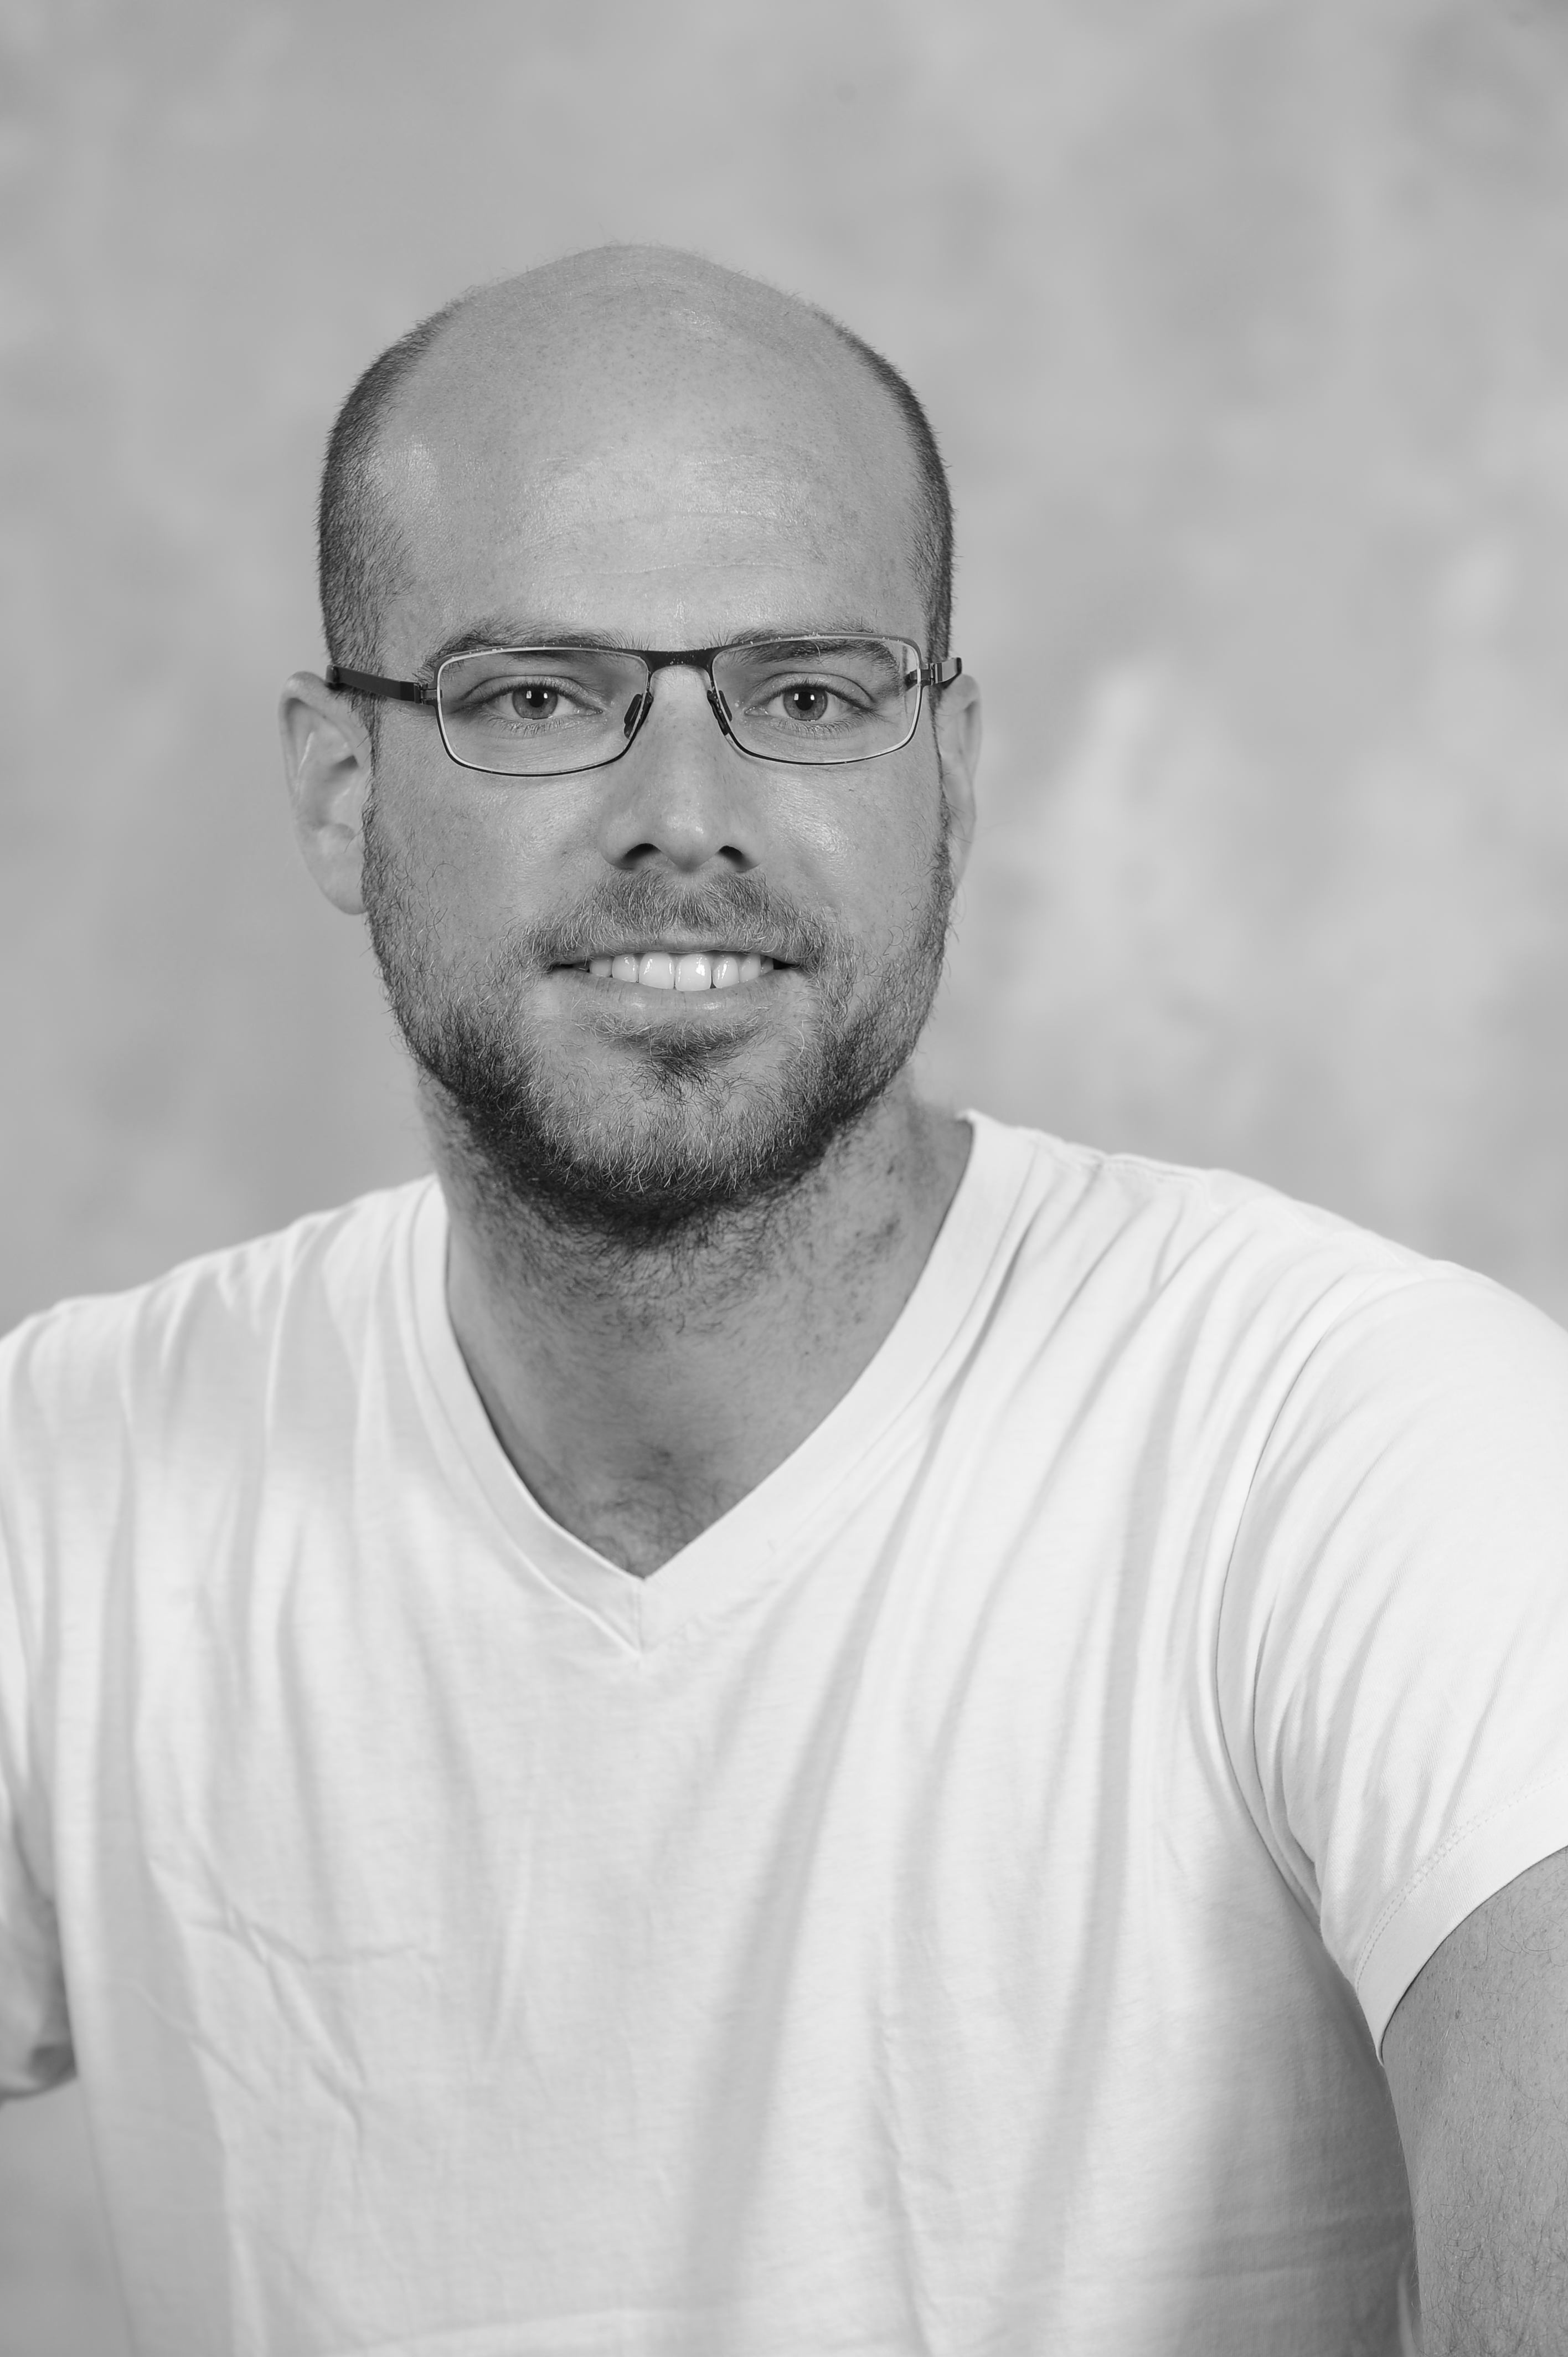
\includegraphics[width=1in,height=1.25in,clip,keepaspectratio]{art/JDR-grey}}]{Jonathan D. Rosenblatt}
is a lecturer at the Industrial Engineering Department in Ben-Gurion University of the Negev, Israel.
His research interests include computational statistics, distributed machine-learning algorithms, spatio-temporal data analysis (fMRI), and high-dimensional signal detection. 
JDR received the Ph.D. degree in Statistics from Tel-Aviv University, and did his post-doc at the Weizmann-Institute of Science. 
He is a member of Ben-Gurion University's Zlotowski Center for Neuroscience.
\end{IEEEbiography}

% if you will not have a photo at all:
\begin{IEEEbiographynophoto}{Yuval Benjamini}
Biography text here.
\end{IEEEbiographynophoto}

% insert where needed to balance the two columns on the last page with
% biographies
%\newpage

\begin{IEEEbiographynophoto}{Roee Gilron}
Biography text here.
\end{IEEEbiographynophoto}


\begin{IEEEbiographynophoto}{Roy Mukamel}
	Biography text here.
\end{IEEEbiographynophoto}


\begin{IEEEbiographynophoto}{Jelle J. Goeman}
	Biography text here.
\end{IEEEbiographynophoto}



% You can push biographies down or up by placing
% a \vfill before or after them. The appropriate
% use of \vfill depends on what kind of text is
% on the last page and whether or not the columns
% are being equalized.

%\vfill

% Can be used to pull up biographies so that the bottom of the last one
% is flush with the other column.
%\enlargethispage{-5in}



% that's all folks
\end{document}


